\section{The Tabu search method}
\subsection{Description of Tabu search methods}
Tabu search is a metaheuristic \footnote{ metaheuristic: simmular to heuristic with the add on that it solves the problem iterativly} optimization method, designed to search for the global optimum. Meaning that the method, figuratively, has the ability to climb out of a local minimum, and then explore other parts of the domain. There are several methods on how these abilities can be acquired. Tabu search uses a so-called tabu list, intended to make already visited areas in the domain forbidden (``tabu''). Tabu search has a few conseptual buildingblocks and basic ideas, easy to understand but widely varying in difficulty to implement. Consepts which, if well implemented, will give you a highly sofisticated search algorithm. The core buildingblock is, as mentioned before, the tabu list. The ability to render certain regions or moves tabu enables us to create search strategys built on the information at hand, both for a given moment and from prior experiences of the search. Hence tabu search is all about coming up with intelligent rules, that will set a specific move to be tabu or not. Another key buildingblock is the tabu overriding mechanism, in literature named as the aspiration criteria [glover]. Its jobb is to check whether a certain move should be approved even if it initially was set to be tabu. In addition this means that the existence of the aspiration criteria allowes the tabu list to be more strict. (And the search a lot faster.)\\
\\
With these two key buildingblocks one can construct almost any type of logic structure. Which makes the tabu search an highly implementable and adaptive method. A logic structure that can be built upon these two concepts is the actual main idea behind the tabu search method. To understand this concept of tabu search one really needs to get on terms with the random aspects of the algorithm.\\
\\The tabu list and aspiration criteria only deals with the random selected \textbf{path/moves/solutions}, this means that the current solution is not necessarily a good one. One of the strengths of the tabu search algorithms is that \emph{any solution produced tells something about the problem at hand, independent of the solutions' quality.} What this really means is that a bad solution also yields important information.  Or, to quote Thomas Edison 
\begin{quotation}
\emph{``I have not failed 1,000 times.  I have
successfully discovered 1,000 ways to NOT make a light bulb.''}
\end{quotation}
This insight might seem somewhat basic at first sight, but if implemented in a good way it yields powerful results.\\
\\In this description certain aspects of the tabu search methods are intentionally neglected. This is in order to make the text more understandable.To gain clairity a generalized tabu search algorithm will described below, in a flow chart and step by step pseudo code.\\
\\
skall laggas in I ordbeskrivnings kappitlet\\
Word convention:\\ 
Complete solution = a set of moves that have solved the problem.\\
Incomplete solution = a set of moves that will not solve the problem.\\
Feasible solution = a set of moves that have not yet solved the problem, or have not yet been evaluated whether it is a complete/incomplete solution.\\

\begin{figure}[!h]
	\centering
	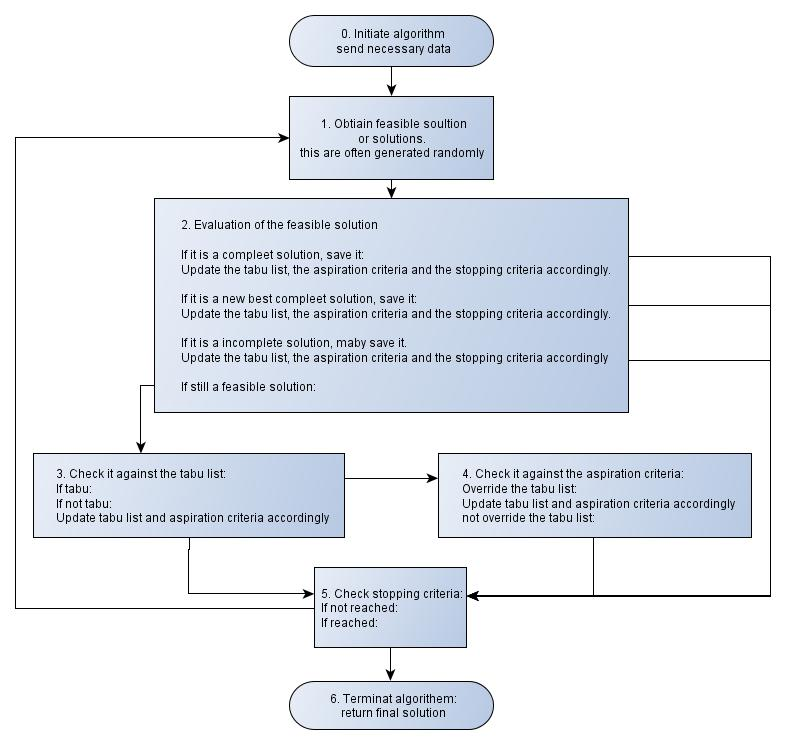
\includegraphics[width=\textwidth]{chapter_4_methods/tabu_generell.jpg}
  	\caption[Generic flow chart of tabu algorithm]
  	{Flow chart of tabu algorithm}
\end{figure}


\subsection{Development process of the Tabu search algorithm}
The developement process of the tabu search algorithm will here be formulated and the choices taken along the road expland. One of the features of this project is that it had a strict deadline. This forced the process in a direction so that the ideas needed to be somewhat easy to implement. \\
\\
Let's start by analysing the random generating of moves a.k.a. feasible solution, see step 1 in figur [flowchart]. The first crossroad was encountered when the decission of generating one feasible solution at a time was taken, instead of generating a set of feasible solutions. The reason behind this choice was that the genetic algorithm already had gone down the path of generating a set of feasible solutions \footnote{ refering to poppulation se sechten???}, since diversity was desired.\\
\\The second crossroad, on the subject of generating moves, was whether to generate one move or a series of moves to generate a new feasible solution. 

This decission was harder to make, since both alternatives seemed to yield highly promising but very different algorithms. The implementation of making a series of moves would be an intermediate between the two choices of the first crossroad. And the result would be a receding horizon [referens johan papper] approach where one had to either:
\begin{itemize}
\item[-]{}Produce a large set of series of moves to later sort by fitness, then choose one to check against the tabu list and aspiration critera.
\item[-]{}Generate a single series of moves to check against the tabu list and aspiration critera.
\end{itemize}

Both alternatives would probably have yielded promising algorithms. But the fact that the tabu list and aspiration critera then would have needed abilities of a more analysing type implied that it would be more difficult to implement. This resulted in that this path was scraped. This meant that the one move one feasible solution approach came out ahead.\\
\\
This settled we can now move forward to view the ideas of the tabu list. In the beginning of the development the ideas flourished. Seven different rules where evaluated:
\begin{enumerate}
\item{}For one feasible solution save the past X number of moves for each pursuer and render these moves tabu to be returned to.
\item{}Do not allow moves that results in X number of lost secured areas.
\item{}Make geometricaly based tabus for critical areas:
\subitem{} Regions of corridor like characteristics would not be needed to be walked down if a pursuer saw its end point or if one had a region with an obstacle that one could walk around. Regions with an obstacle of that kind would need two pursuers to be secured, thus it would be tabu to go about and try to secure it alone. And finaly if one hade a tree like corridor system, going about to solve it would only be allowed with the right amount of pursuers.
\item{} Work togheter:
\subitem{} Somewhat similar to tabu rule (3), but with the addon that two pursuers never really need to see each other only share vissible areas. This is  a more general rule that would need to be weighted in the aspriation criteria.
\item{} High valued areas:
\subitem{} Trying to incorporate the idea of getting information even from bad solutions. This would be made by considering the path taken, areas walked upon in a complete solution should be given a value bonus. Or if you look upon it from another angle, areas not walked upon could be set to be tabu. 
\item{} Low valued areas:
\subitem {}An incomplete solution may have a series of moves that have been concentrated on a specific region for to long, hence one could give this areas a value penalty.
\item{} Not alow, or give value penaltys to moves in already secured areas.
\end{enumerate}

All these tabus needed to be ranked, given a priority level that would be weighted in the aspiration criteria. Also many of the tabu rules listed above needed some sort of worst case senario handeling, to avoid that the algorithm would get stuck.\\
\\This said, let's now diskuss the aspiration critera:
As understood from the text above the aspiration critera needs to incorporate a lot. As a start it needs to have the ability of checking wheter an area is of high or low value. Which then means that the evaluation step in figure [flochart1] needs a fitness calculation function that would depend on the area visited and the shape of the feasible solution. Sad to say this aspiration criteria, would need an overwhelming amount of work to implement. Thus this advanced aspiration criteria was scrapped for a simpler one. This also means that tabu rules (3), (4), (6) and (7) no longer could be implemented. Tabu rule (5) got simplified to:  areas not walked upon where set to be tabu. More about tabu rule (5) later. The more simple aspiration criteria, in the end, only came to be: more of a worst case scenario handling, to avoid the algorithm of getting stuck.\\
\\Tabu rule (5): When this rule first was implemented the idea was that X number of past complete solutions were analysed to check which areas had been walked upon at least once, and render the rest tabu. The problem was however that this wasn't strict enough. So X was set to one. Which in turn led to a new problem. The problem that arouse was that the algorithm now, under certain circumstances, was too hasty in returning a final solution. This was partially solved by a new stoping criteria and ``go about it again criteria''.\\
\\
That was the development process of the tabu search algorithm, the final version can be viewed in figure [ ] and is also discussed in the next section.\\
\subsection{The Tabu search algorithm for our problem}
%kollat hit!
%kollat hit.
%kollat hit.
%kollat hit.
%kollat hit.
The tabu search algorithm used for solving the problem be discussed here.\\
In figur [generella tabu] a generall step by step explanation was made of the tabu search algorithm. In figur [???] a modified version can be seen, intended to illustrate the final algorithm and also to show what functions from to the general algorithm that was removed.\\

\begin{figure}[!h]
	\centering
	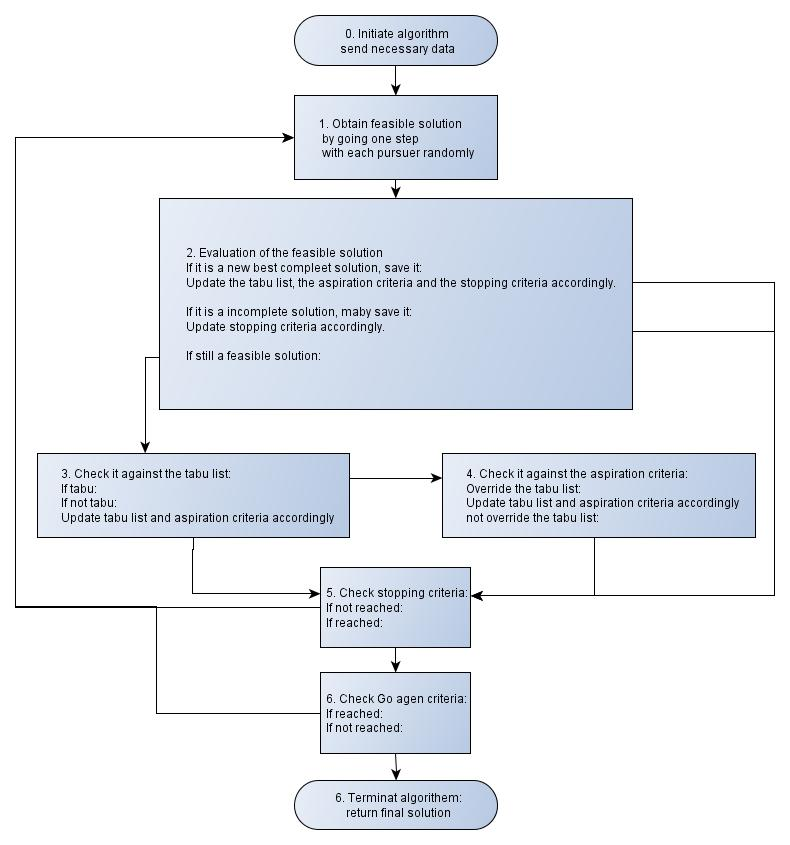
\includegraphics[width=\textwidth]{chapter_4_methods/tabu_ny.jpg}
  	\caption[Final algorithm flow chart of tabu algorithm]
  	{Final algorithm flow chart of tabu algorithm}
\end{figure}

To get a feel for the algorithm and to point out insufficiencys, an explanation of how the algorithm converges is in order.\\
There are two elements in the algorithm that affect the convergens:
\begin{enumerate}
\item{} Tabu roule (5)
\item{} Best-solution-found-so-far stopping criteria. 
\subitem{} Mening that if a solution is found one does not search for a solution with a path of longer length.
\end{enumerate}
To note here is that both convergens helping elements depend on that they actualy hava a complete solution. Meaning that if the algorithm is unlucky in finding the first complete solution, the computational time will rise acordingly. As a said note, this considerable insufficiency migth have been avoided with the more advansed aspiration critera, discussed in section [develupment].

\subsection{Implementation of the Tabu search algorithm}
In this section two important aspects of the implementation will be discussed. These two are obvious shortcomings in the algorithm and parameter values. With the implementation, a series of parameter values arouse. Parameter values that had three different features:
\begin{enumerate}
\item{} Tabu rule values:
\begin{enumerate}
\item{} Tabu rule (1)  save\_past\_X\_number\_of\_moves 
\item{} Tabu rule (2)  X\_number\_of\_lost\_secured\_areas
\end{enumerate} 
\item{} Aspiration criteria values:
\begin{enumerate}
\item{} Override\_X\_number\_of\_lost\_secured\_areas
\item{} Override \_save\_past\_X\_number\_of\_moves
\end{enumerate} 
\item{} Stopping criteria values:
\begin{enumerate}
\item{} Max\_incomplete\_solutions\_ found \_in\_a\_row
\item{} Max\_ equal\_complete\_solutions\_ found \_in\_a\_row
\item{} Max\_allowed\_steps
\end{enumerate} 
\item{} Go again values:
\begin{enumerate}
\item{} Restart\_the\_algorithm\_X\_times
\item{} Restart\_the\_algorithm\_X\_times\_keep\_best\_complete\_solution
\item{} X\_steps\_is\_this\_realy\_the\_best\_complet\_solution
\end{enumerate} 
\end{enumerate} 
As can be seen in the list above some of the parameters have strong relations to eachother. These relations will now be explained. Parameter values (1) and (2) are related in a way so that (2) ensures that (1) does not make the algorithm freeze. Parameter value (4.2) and (4.3) aims to avoid the algorithm from being to hasty in returning a final solution, when encountering a less difficult enviroment. The Max\_allowed\_steps and Restart\_the\_algorithmen\_X\_times tries to tackle the problem of finding the first complete solution. The computational time, and the probability of finding any solution at all, totally depends on this relation. As discussed lastly in section 4.2.3 the algorithms' computational time will be affected if the first complete solution is found at a late stage in the search. But the computational time will be even greater affected if one wants to increase the probability the finding of a solution at all. Meaning that if The Max\_allowed\_steps value is increased, the chances of finding a complete solution should increase. Parameter value (3.1) and (3.2) has two properties, first to terminate the algorithm and secondly to not terminate the algorithm until the search space has been throughly examined in promising regions. Parameter (3.2) is also an indicator of that the the search has converged to a certain final solution.\\
\\
\indent Obvious shortcomings in the algorithm:\\
Mera text
